The primary objective of this thesis is to implement and assess the potentials and limitations of integrating LLM-based Automated Bug Fixing into Continuous Integration. We aim to answer the following research questions to evaluate the system's capabilities and impact on the software development process:

\begin{itemize}
    \item \textbf{RQ1:} How can LLM-based automated bug fixing be effectively and efficiently integrated into a CI pipeline?
    \item \textbf{RQ2:} What are the potentials and limitations of this integrated approach in terms of repair success rate, cost-effectiveness and developer workflow enhancement?
\end{itemize}

To answer these questions, we streamlined the process into three phases: preparation, implementation/usage, and evaluation. The process is visualized below in Figure \ref{fig:method-overview}.

\begin{figure}[H]
    \centering
    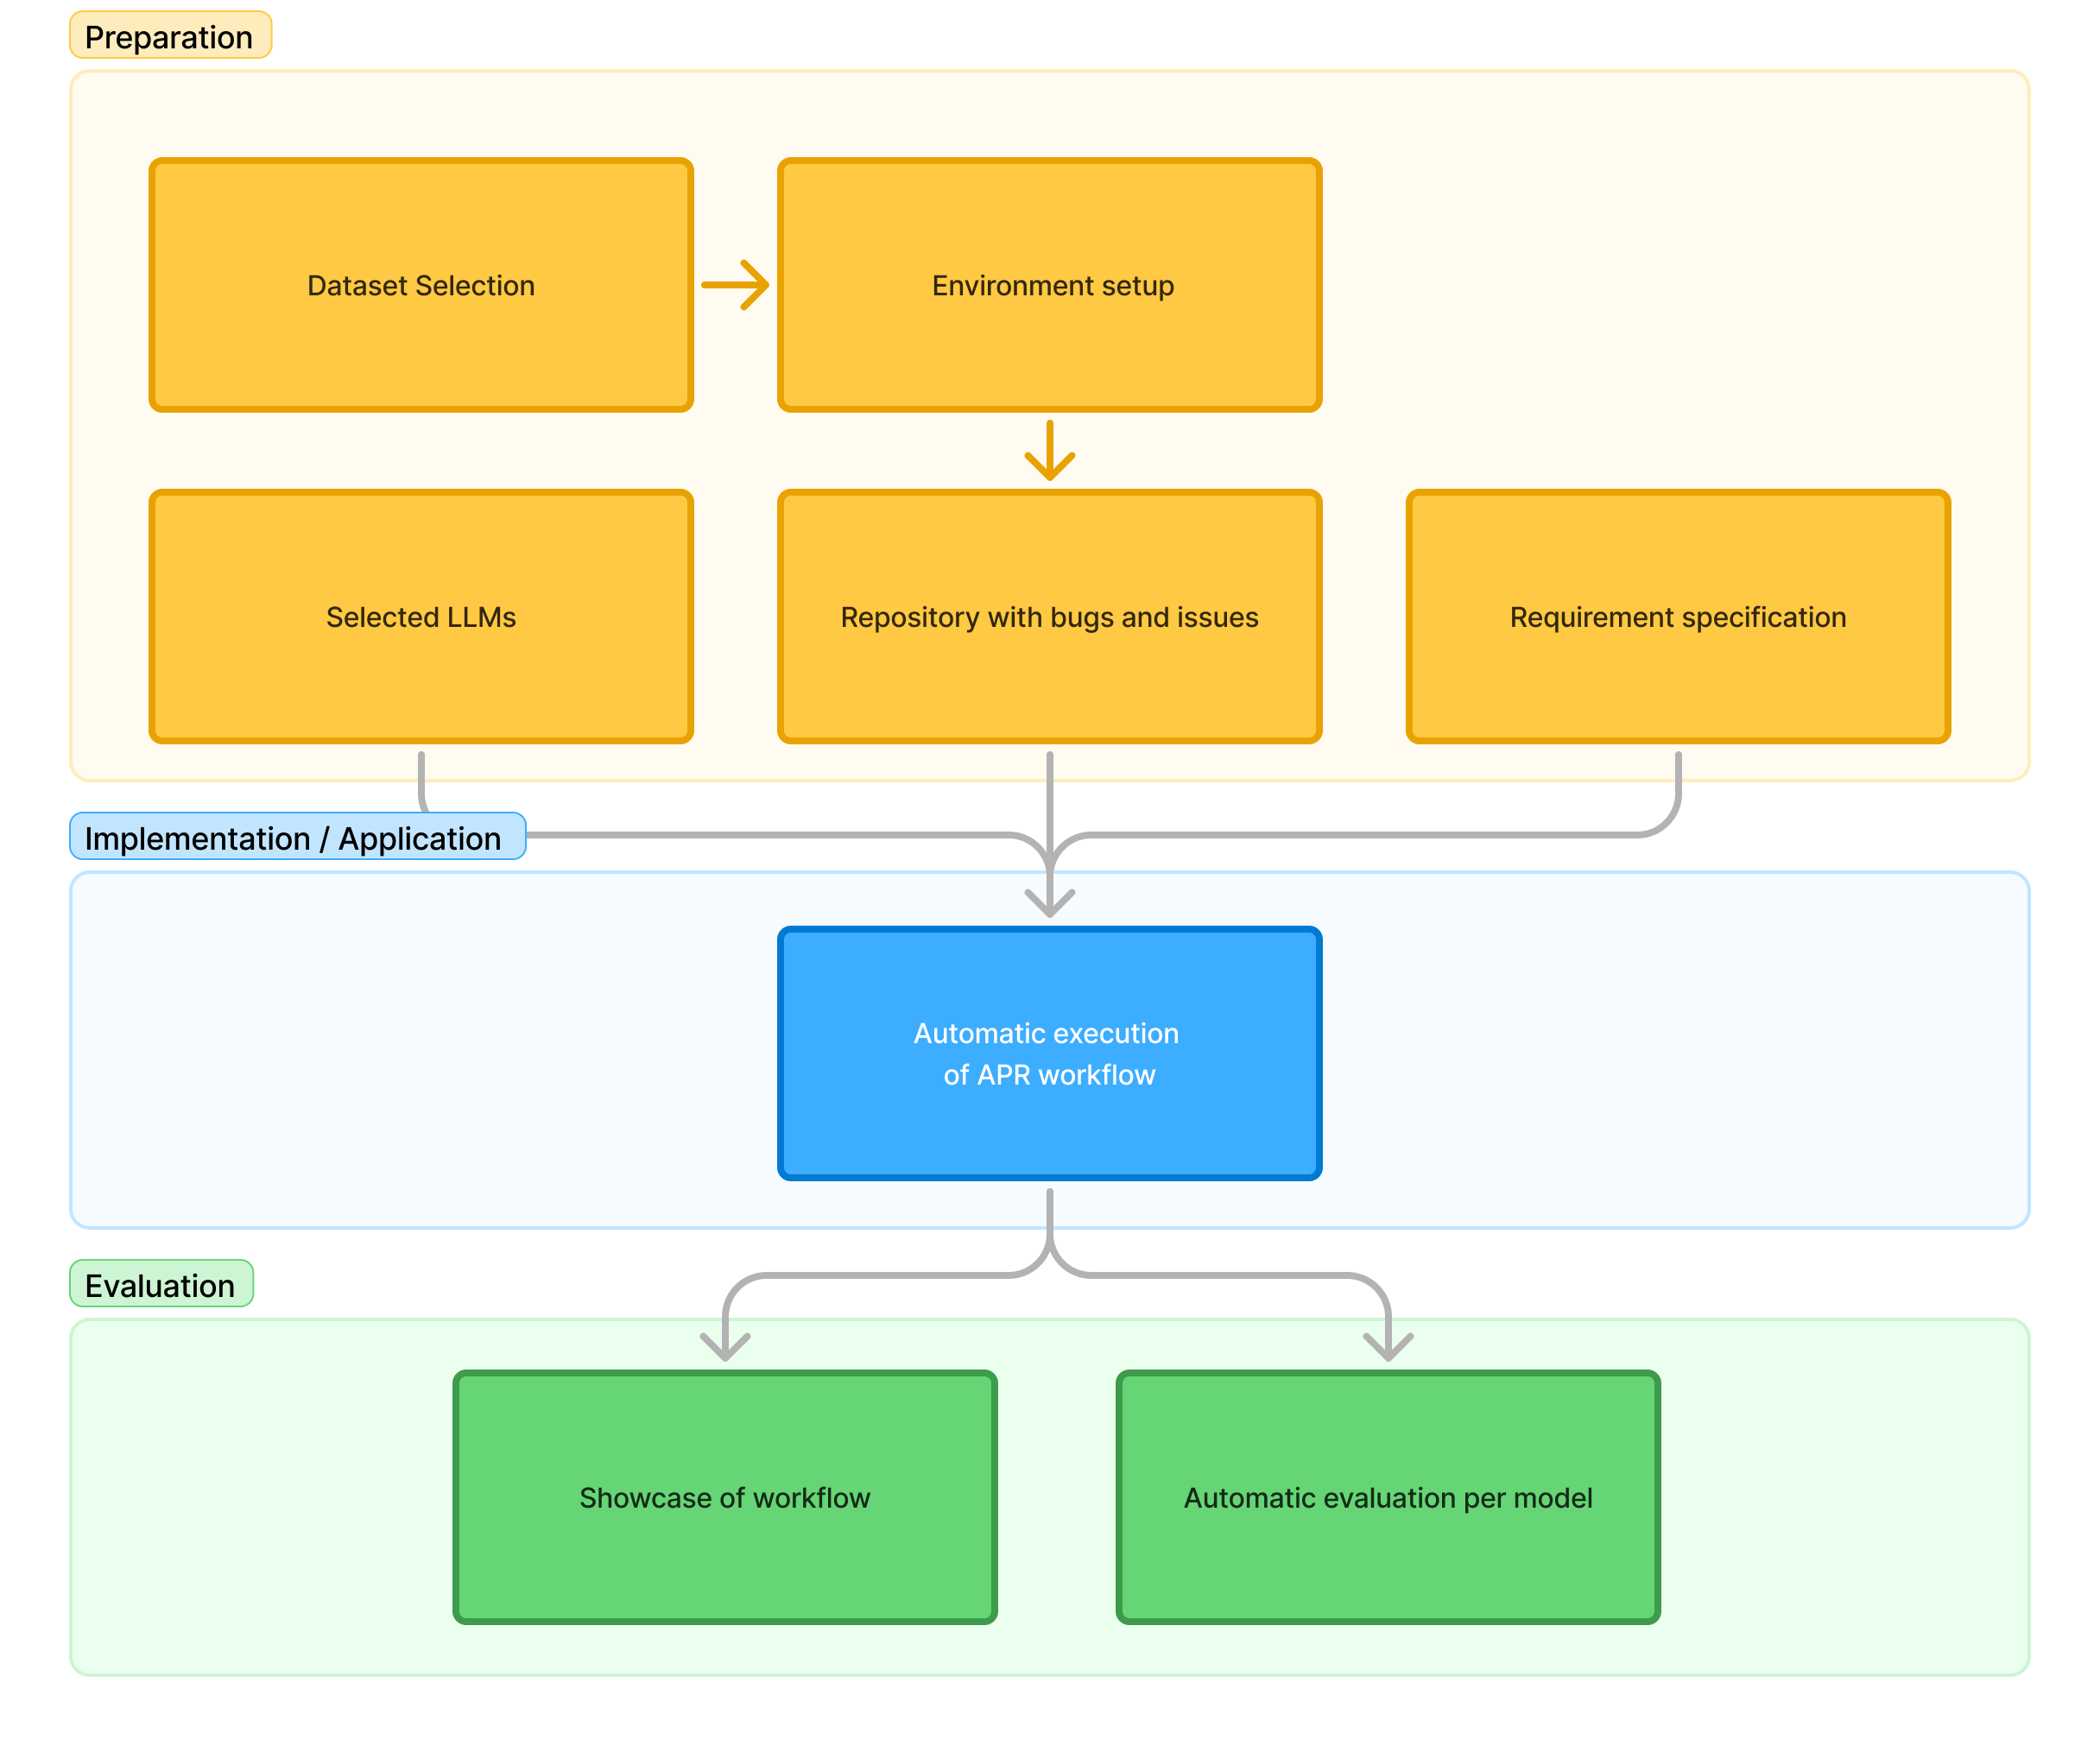
\includegraphics[width=1\textwidth]{images/flowcharts/method.png}
    \caption{Thesis methodology approach}
    \label{fig:method-overview}
\end{figure}

In the preparation phase, we select a suitable APR benchmark and a pool of LLMs. With the benchmark, we set up a realistic development environment. By specifying requirements, we lay the groundwork for the implementation of the APR system.
In the second part, we implement the APR system as a GitHub Action workflow based on the requirements.
Lastly, we evaluate the self-developed prototype using the defined evaluation metrics \ref{section:evaluation} collected during and after the execution of the APR system. Furthermore, we showcase the resulting workflow of using the system in the prepared repository.
The following sections will go into detail about each of these phases.

\section{Preparation}

For implementing and evaluating our system, we first need to prepare an environment where the system can be integrated, used, and evaluated. This includes selecting a suitable dataset and Large Language Models, setting up the environment, and specifying the requirements for the system.

\subsection{Dataset Selection}

For evaluating the effectiveness of our APR integration, we selected the QuixBugs benchmark \cite{linQuixBugsMultilingualProgram2017}. This dataset is well-suited for our purposes due to its focus on small-scale bugs in Python\footnote{The QuixBugs benchmark contains the same bugs translated to Java as well. We will exclude this for evaluation research}. It consists of 40 individual files, each containing an algorithmic bug. Each bug is caused by a single erroneous line. Corresponding tests and a corrected version for every file are also included in the benchmark, which allows for seamless repair validation. QuixBugs was developed as a set of challenging problems for developers \cite{linQuixBugsMultilingualProgram2017}, enabling us to evaluate whether our system can take over the cognitively demanding task of fixing small bugs without developer intervention.

Additionally, compared to other APR benchmarks \ref{table:benchmarks} like SWE-Bench \cite{jimenezSWEbenchCanLanguage2024}, QuixBugs is relatively small, which allows for accelerated setup and development.

\subsection{LLM Selection} \label{subsection:llm-selection}

For the evaluation of our APR system, we will test a selected pool of LLM models. We evaluate with the latest models released before 11 July 2025 from the three vendors that currently dominate AI-assisted coding workflows: Google, OpenAI, and Anthropic. The models are selected to cover a range of capabilities and costs, with a focus on lower-tier models, allowing us to evaluate the performance and cost-effectiveness of the APR system. Table \ref{table:llms} shows the selected models that will be used for evaluation with the following data:

\begin{itemize}
    \item (1) Model Name: The name of the LLM model.
    \item (2) Publisher: The company or organization that developed the model.
    \item (3) Context Window Size in Tokens: The maximum number of tokens the model can process in a single request.
    \item (4) Cost per 1M Tokens: The cost of processing 1 million tokens, divided into input and output cost.
    \item (5) Provider Description: Description of the model's characteristics.
\end{itemize}

\begin{longtable}{@{\extracolsep{\fill}}  p{4cm} | p{2cm} | p{2cm} | p{2.5cm} | p{2.5cm} @{}}
    \caption{Characteristics of selected LLMs (21.07.2025)} \label{table:llms}                                     \\

    \hline
    \textbf{(1)}                      & \textbf{(2)} & \textbf{(3)} & \textbf{(4)}                  & \textbf{(5)} \\
    \hline
    \endfirsthead

    \hline
    \endfoot
    \textbf{gemini-2.0-flash-lite}    & Google       & 1,048,576    & input: \$0.075 output: \$0.30 & X            \\ \hline
    \textbf{gemini-2.0-flash}         & Google       & 1,048,576    & input: \$0.15 output: \$0.60  & X            \\ \hline
    \textbf{gemini-2.5-flash-preview} & Google       & 1,000,000    & input: \$0.10 output: \$0.40  & X            \\ \hline
    \textbf{gemini-2.5-flash}         & Google       & 1,048,576    & input: \$0.30 output: \$2.50  & X            \\ \hline
    \textbf{gemini-2.5-pro}           & Google       & 1,048,576    & input: \$1.25 output: \$10.00 & X            \\ \hline
    \textbf{gpt-4.1-nano}             & OpenAI       & 1,047,576    & input: \$0.10 output: \$0.40  & X            \\ \hline
    \textbf{gpt-4.1-mini}             & OpenAI       & 1,047,576    & input: \$0.40 output: \$1.60  & X            \\ \hline
    \textbf{gpt-4.1}                  & OpenAI       & 1,047,576    & input: \$2.00 output: \$8.00  & X            \\ \hline
    \textbf{o4-mini}                  & OpenAI       & 200,000      & input: \$1.10 output: \$4.40  & X            \\ \hline
    \textbf{claude-3-5-haiku}         & Anthropic    & 200,000      & input: \$0.80 output: \$4.00  & X            \\ \hline
    \textbf{claude-3-7-sonnet}        & Anthropic    & 200,000      & input: \$3.00 output: \$15.00 & X            \\ \hline
    \textbf{claude-sonnet-4-0}        & Anthropic    & 200,000      & input: \$3.00 output: \$15.00 & X            \\
    \hline
\end{longtable}


\subsection{Environment Setup} \label{subsection:environment-setup}
To mirror a realistic software development environment, we prepared a GitHub repository containing the QuixBugs Python dataset. This repository serves as the basis for the bug-fixing process, allowing the system to interact with the codebase and perform repairs.

Using the relevant 40 files, we generate a GitHub issue for each bug. A consistent issue template is used, capturing only the title of the problem with a minimal description. The generated issues serve as the entry point and communication medium for the APR system. Figure \ref{fig:gh-issue} shows an example of a generated GitHub issue.

\begin{figure}[H]
    \centering
    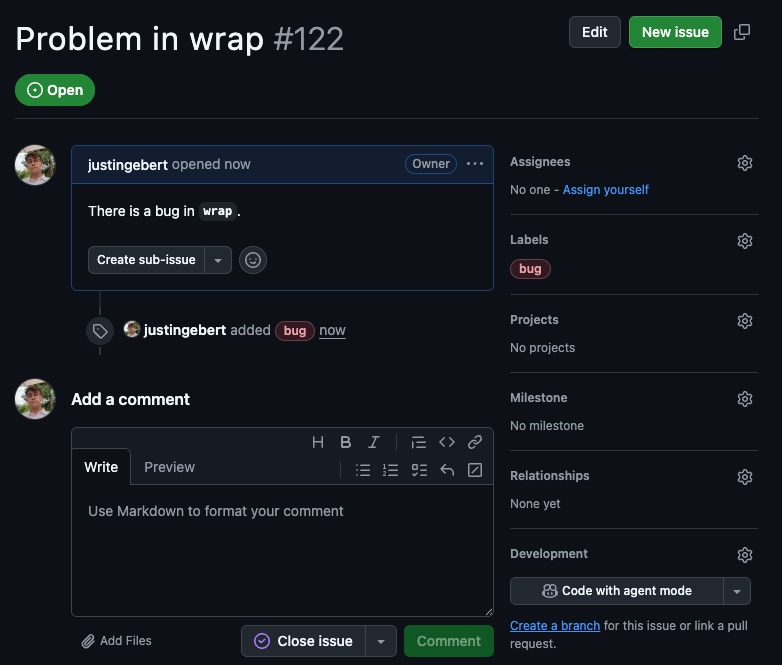
\includegraphics[width=1\textwidth]{images/github/github_issue.png}
    \caption{Example of a generated GitHub Issue}
    \label{fig:gh-issue2}
\end{figure}

\subsection{Requirements Specification}

Before the implementation phase, we constructed requirements for the prototype, applying the INVEST model, a widely adopted method in Agile software development for engineering requirements \cite{10.5555/984017}. According to the INVEST principles, each requirement was formulated to be independent, negotiable, valuable, estimable, small, and testable. Using this framework, we defined both functional and non-functional requirements. The requirements are precisely defined, verifiable, and easily adaptable to iterative development. The resulting requirements are detailed in \ref{chapter:requirements}.

\section{System Implementation}

In this section, we provide a high-level overview of the implemented Automated Bug Fixing Pipeline. A detailed implementation description can be found in \ref{chapter:implementation}.

The Automated Bug Fixing Pipeline was developed using iterative prototyping and testing, with a focus on simplicity and extensibility. Based on the self-developed requirements \ref{chapter:requirements}, we built the system visualized in Figure \ref{fig:high-level} and Figure \ref{fig:apr-core-overview}.

The integration of the pipeline into the repository is performed during this implementation phase. Once the system is in place, the pipeline can be triggered by different events. This executes the CI pipeline on a GitHub Action runner. The first pipeline job fetches and filters relevant issues. Resulting issues are passed to the APR Core, which contains the main bug-fixing logic. The APR Core runs in a container and communicates with the configured LLMs via API to localize and fix the issue. With the generated file edits, the changes are validated and tested. When validation passes, the changes are applied and a Pull Request is opened on the repository, linking the issue and providing details about the repair process. In case of an unsuccessful repair or exhaustion of the maximum number of attempts, a failure is reported to the issue.

\begin{figure}[H]
    \centering
    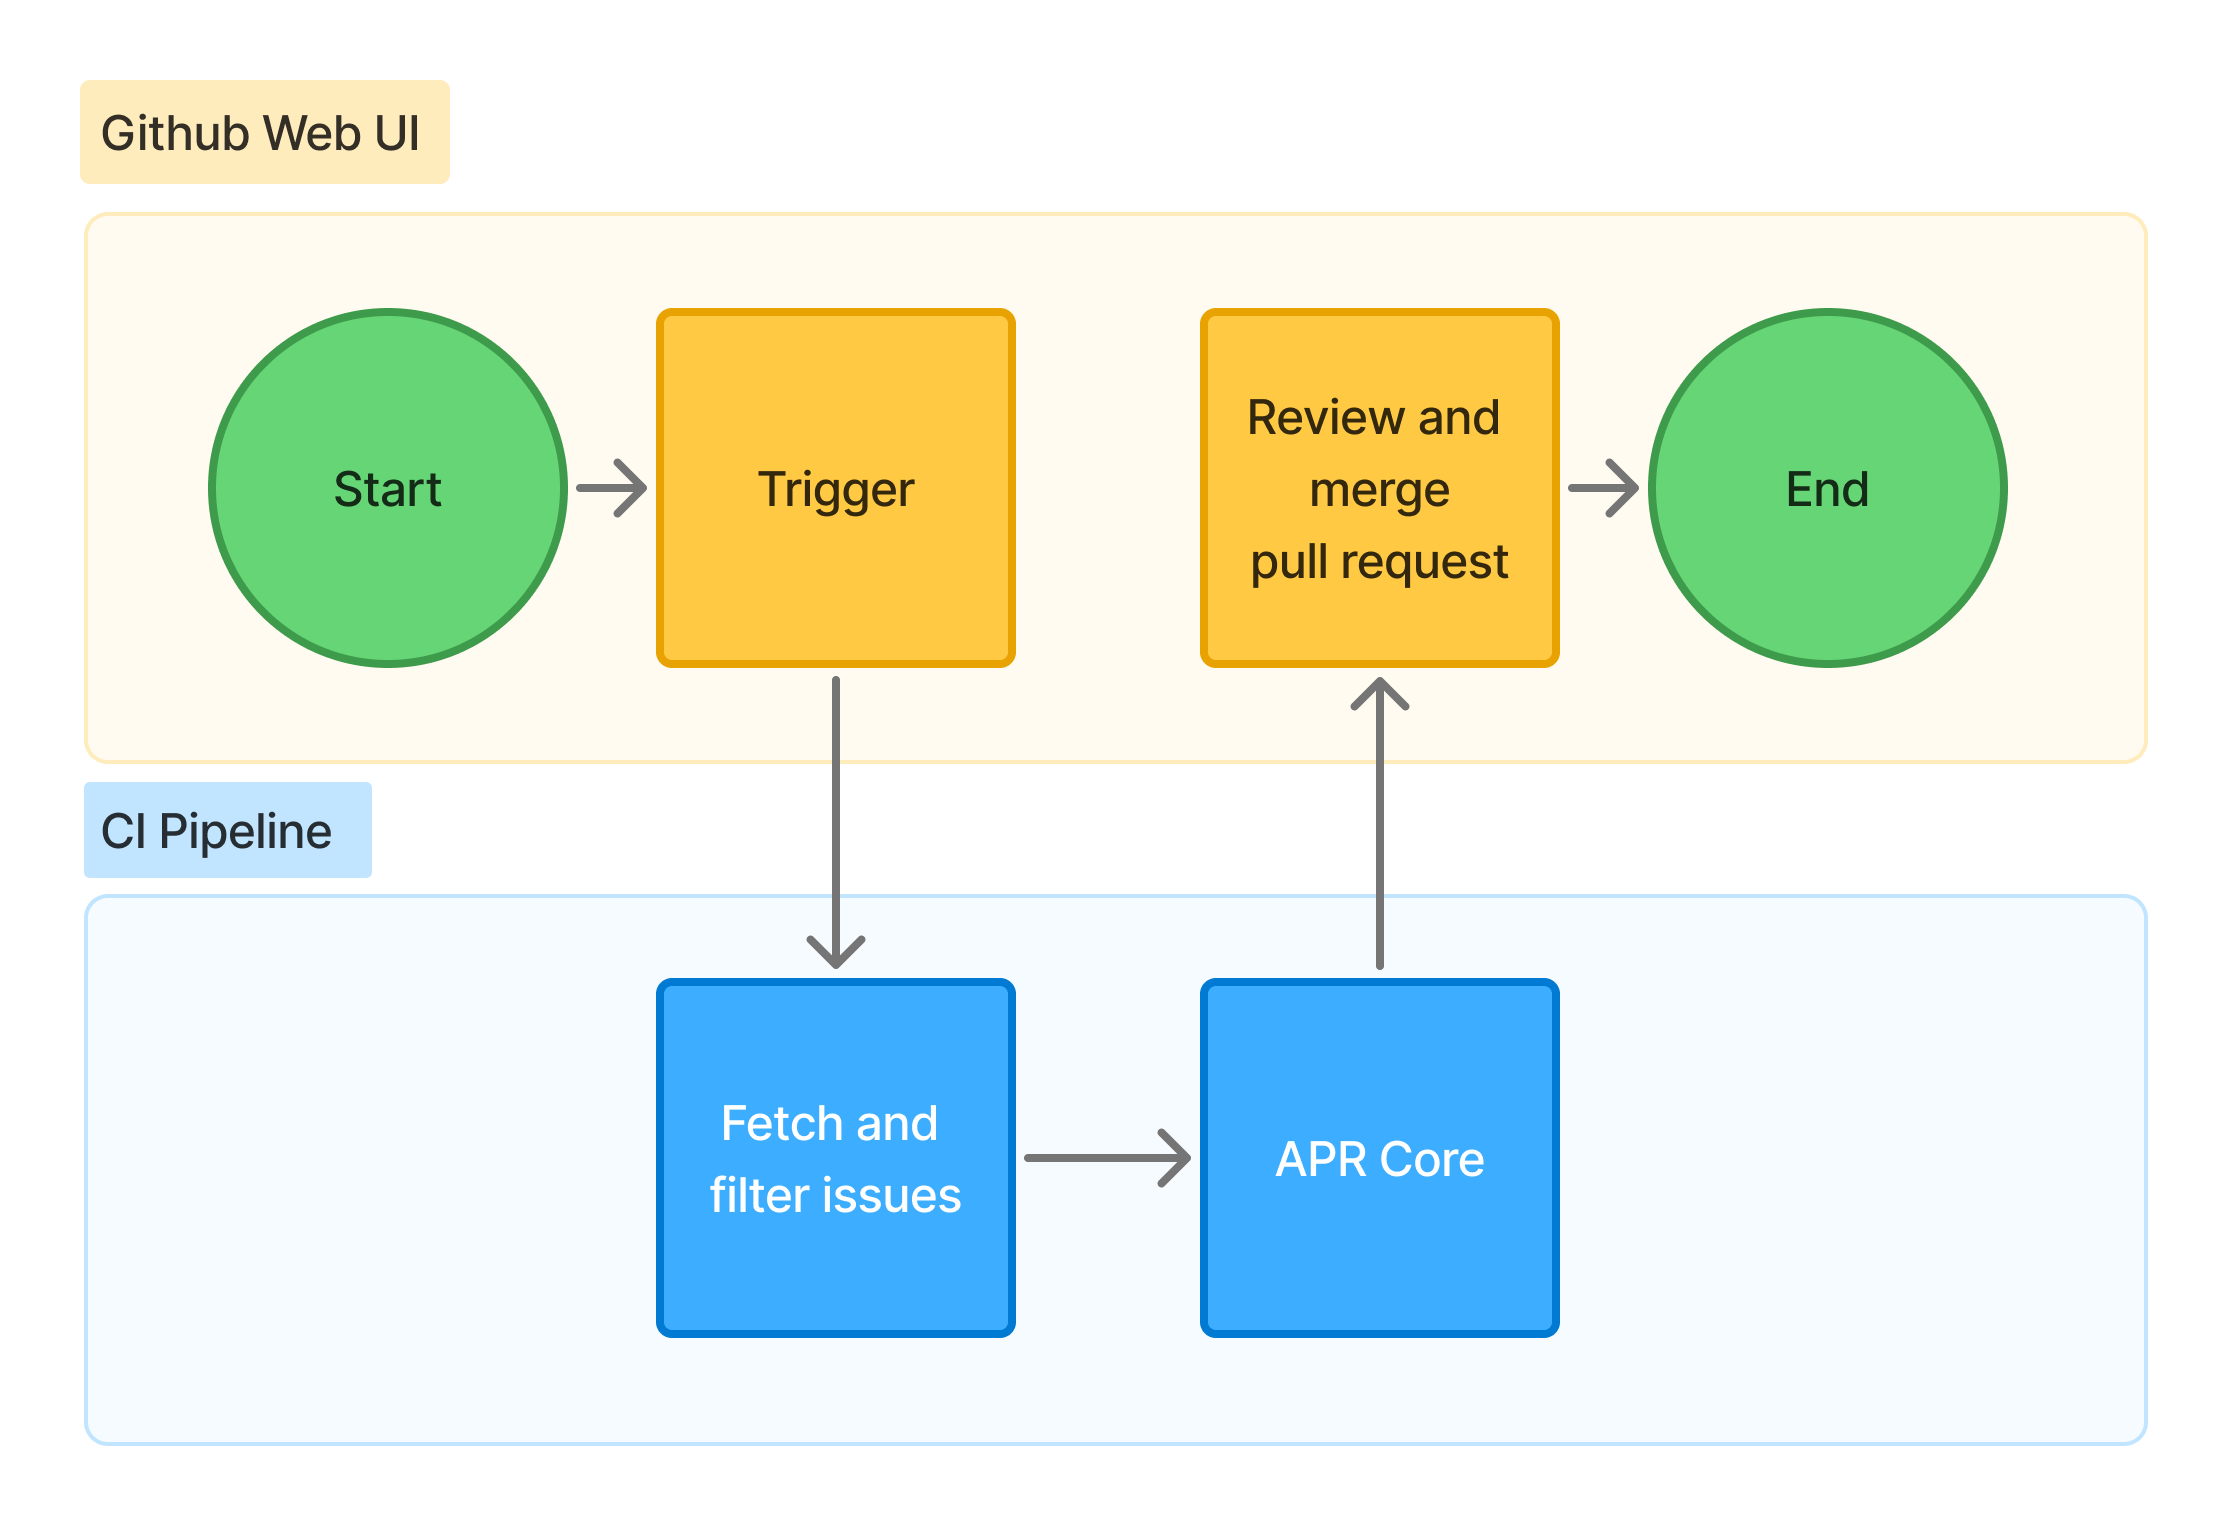
\includegraphics[width=1\textwidth]{images/flowcharts/overview.png}
    \caption{Overview of the APR Pipeline}
    \label{fig:high-level}
\end{figure}

\begin{figure}[H]
    \centering
    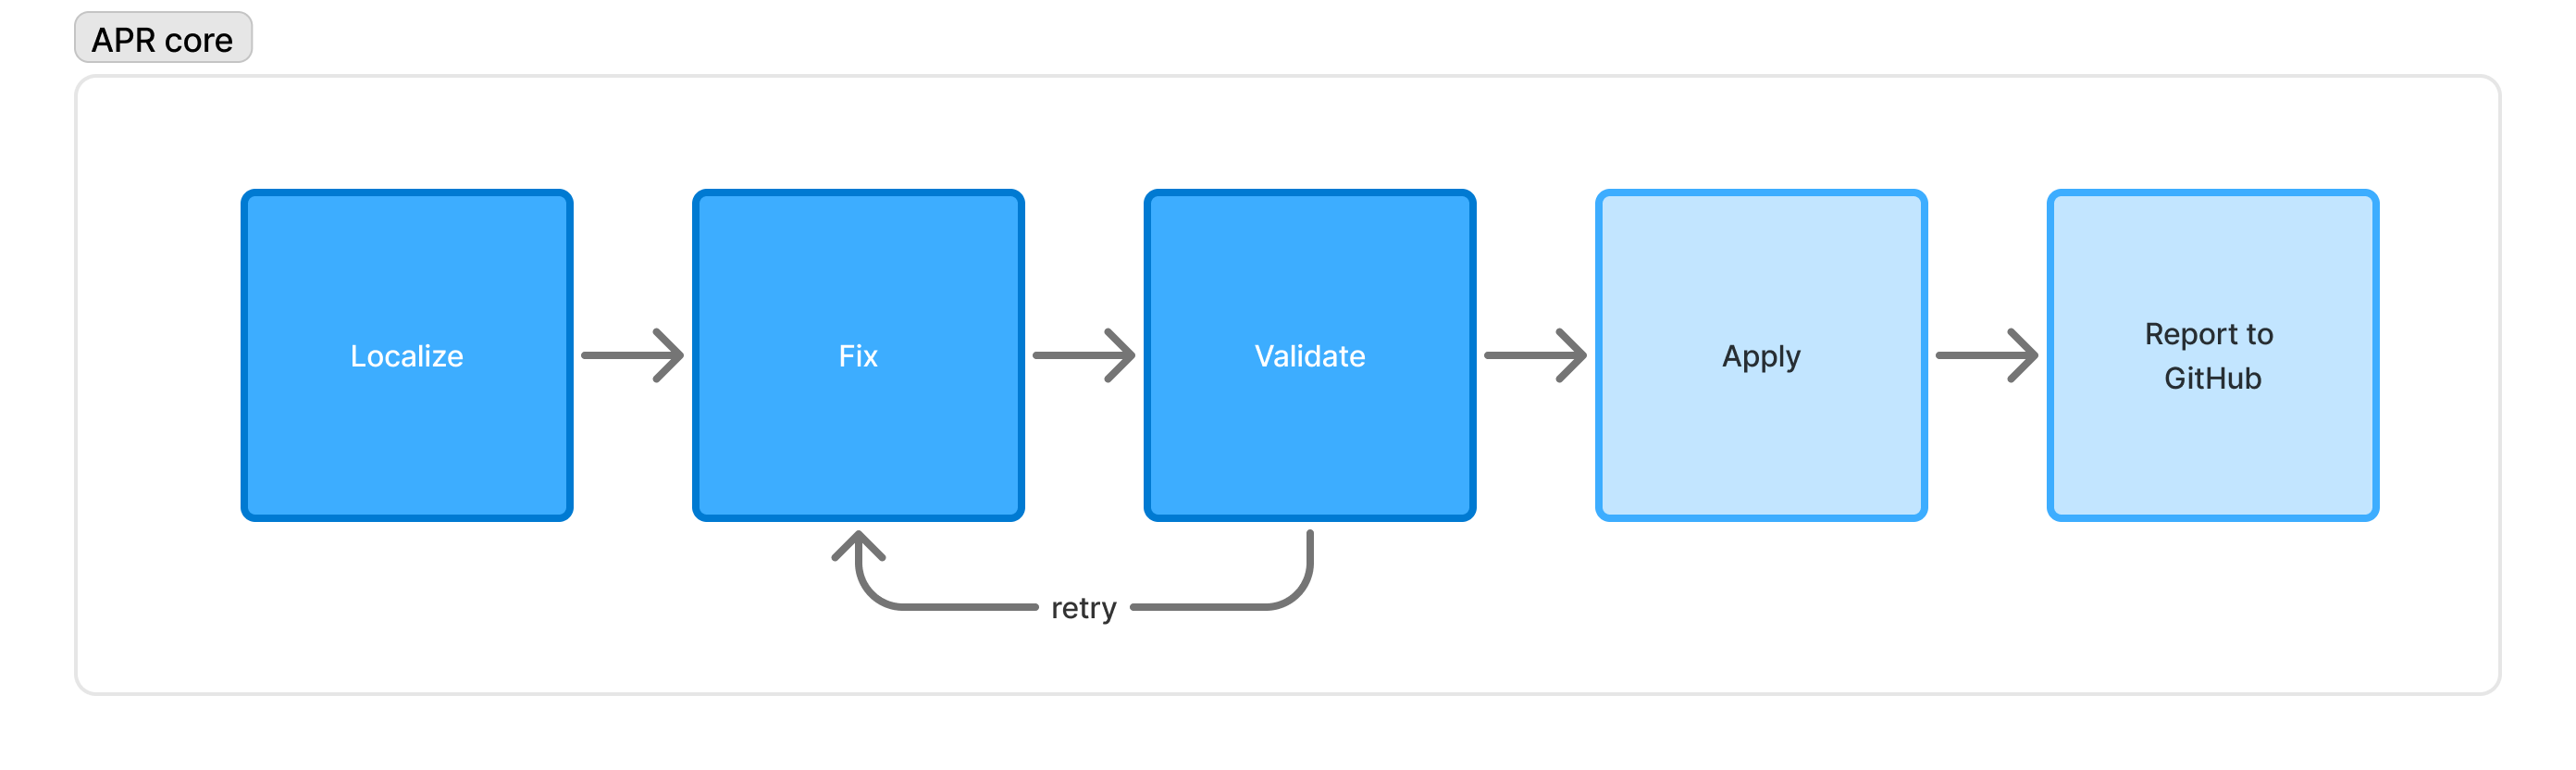
\includegraphics[width=1\textwidth]{images/flowcharts/apr_core_overview.png}
    \caption{Overview of the APR Core}
    \label{fig:apr-core-overview}
\end{figure}



\section{Evaluation} \label{section:evaluation}
%TODO should I mention showcase of results here?
In this section, we describe how we measure the effectiveness, performance, and cost of the APR pipeline when integrated into a GitHub repository. We use GitHub Actions' Continuous Integration capabilities in combination with the prepared QuixBugs repository as a base. All selected LLM models from table \ref{subsection:llm-selection} are evaluated in the context of the APR system. The evaluation is based on data collected during and after the execution of the APR pipeline.

We focus on several key data metrics to assess the system's performance and capabilities in repairing software bugs. These metrics provide insights into the system's effectiveness, performance, reliability, cost, and overall impact on the software development lifecycle.

To evaluate the effectiveness of the LLM models and the approach, we determine a repair success rate. A successful repair of an issue is determined by validation and the complete test suite provided by QuixBugs. An issue is considered successfully repaired when the validation passes with correct syntax and the related test suite passes all tests.

Furthermore, we evaluate whether multiple attempts can help improve the repair success rate and how this relates to the cost of the repair process.

To assess performance, we analyze collected fine-grained timings of issue repair attempts. Feasibility is evaluated by estimating the cost of a repair attempt based on the number of tokens and token pricing listed by API providers. GitHub Action run minutes are not included in the cost estimation, as 2000 minutes are included in the free tier of GitHub for public repositories.

The following data is automatically collected by each run of the APR system. Using self-developed scripts, we collect the data from different sources for each run. Below, we list the relevant data collected for each run \ref{table:run-metrics}, each issue processed \ref{table:issue-metrics}, and each stage of an issue repair process \ref{table:stage-metrics}. We use the collected data to calculate results for different runs testing each of the selected models, which will help in answering RQ2. The calculations are listed in Table \ref{table:calculations}.

%TODO add calculations and check if all metrics are needed or evaluation
\begin{table}[ht]
    \centering
    \small
    \renewcommand{\arraystretch}{1.5}
    \begin{tabular*}{\textwidth}{@{\extracolsep{\fill}} p{3.2cm} | p{7cm} | p{3.5cm} @{}}
        \hline
        \textbf{Metric} & \textbf{Description} & \textbf{Source} \\
        \hline
        Run ID & Unique identifier for the workflow run & Github Action Runner \\ \hline
        Configuration & Configuration details, including LLM Model used and max attempts & Github repository / APR Core  \\ \hline
        Execution Time & Total time taken for the run & GitHub API / APR Core \\ \hline
        Job Execution Times & Time taken for each job in the pipeline & Github API \\ \hline
        Issues Processed & Data of issues processed shown in table \ref{table:issue-metrics} & APR Core \\
        \hline
    \end{tabular*}
    \caption{Summary of metrics collected for each run}
    \label{table:run-metrics}
\end{table}

\begin{table}[H]
    \centering
    \small
    \renewcommand{\arraystretch}{1.5}
    \begin{tabular*}{\textwidth}{@{\extracolsep{\fill}} p{3.2cm} | p{7cm} | p{3.5cm} @{}}
        \hline
        \textbf{Metric} & \textbf{Description} & \textbf{Source} \\
        \hline
        Issue ID & Unique identifier of the issue & Github Issue ID \\ \hline
        Repair Successful & Boolean indicating whether the repair was successful & APR Core \\ \hline
        Number of Attempts & Total attempts made & APR Core \\ \hline
        Execution Time & Time taken to process the issue, including all stages & APR Core \\ \hline
        Tokens Used & Number of tokens processed by the LLM during the repair process & LLM API \\ \hline
        Cost & Cost associated with the repair process, calculated based on tokens * cost per token & APR Core \\ \hline
        Stage Information & Details about each stage of the repair process shown in table \ref{table:stage-metrics} & APR Core \\
        \hline
    \end{tabular*}
    \caption{Summary of metrics collected for each processed issue}
    \label{table:issue-metrics}
\end{table}

\begin{table}[H]
    \centering
    \small
    \renewcommand{\arraystretch}{1.5}
    \begin{tabular*}{\textwidth}{@{\extracolsep{\fill}} p{3.2cm} | p{7cm} | p{3.5cm} @{}}
        \hline
        \textbf{Metrics} & \textbf{Description} & \textbf{Source} \\
        \hline
        Stage ID & Unique identifier of the stage & APR Core \\ \hline
        Stage Execution Time & Time taken for stage to complete & APR Core \\ \hline
        Stage Outcome & Outcome of each stage, indicating success, warning or failure & APR Core \\ \hline
        Stage Details & Additional details, such as error or warnings messages & APR Core \\
        \hline
    \end{tabular*}
    \caption{Summary of metrics collected for each stage}
    \label{table:stage-metrics}
\end{table}

\begin{table}[H]
    \centering
    \small
    \renewcommand{\arraystretch}{1.5}
    \begin{tabular*}{\textwidth}{@{\extracolsep{\fill}} p{5cm} | p{10cm} @{}}
        \hline
        \textbf{Metrics} &  \textbf{Calculation} \\
        \hline
        Repair Success Rate & \[\frac{Number of Successful Repairs}{Total Issues Processed}\] \\ \hline
        Average Execution Time per Issue & \[\frac{Total Execution Time}{Total Issues Processed}\] \\ \hline
        Average Cost per Issue& \[\frac{Total Cost}{Total Issues Processed}\] \\ \hline
        APR Core Execution Time & \[\frac{Total APR Core Execution Time}{Total Issues Processed}\] \\ \hline
        CI Pipeline Execution Time & \[\frac{Total CI Pipeline Execution Time}{Total Issues Processed}\] \\ \hline
        \hline
    \end{tabular*}
    \caption{Run evaluation metrics calculated from the collected data}
    \label{table:calculations}
\end{table}
